\documentclass[12pt, a4paper, oneside]{ctexart}
\usepackage{amsmath, amsthm, amssymb, bm, color, graphicx, geometry, mathrsfs,extarrows, braket, booktabs, array}
\usepackage[colorlinks,linkcolor=red,anchorcolor=blue,citecolor=blue,urlcolor=blue,menucolor=black]{hyperref}
%%%% 设置中文字体 %%%%
\setCJKmainfont{方正新书宋_GBK.ttf}[ BoldFont = 方正小标宋_GBK, ItalicFont = 方正楷体_GBK]
%%%% 设置英文字体 %%%%
\setmainfont{Times New Roman}
\setsansfont{Calibri}
\setmonofont{Consolas}

\linespread{1.4}
%\geometry{left=2.54cm,right=2.54cm,top=3.18cm,bottom=3.18cm}
\geometry{left=1.84cm,right=1.84cm,top=2.18cm,bottom=2.18cm}
\newcounter{problem}  % 问题序号计数器
\newenvironment{problem}{\stepcounter{problem}\par\noindent\textbf{题目\arabic{problem}. }}{\smallskip\par}
\newenvironment{solution}{\par\noindent\textbf{解答. }}{\smallskip\par}
\newenvironment{note}{\par\noindent\textbf{注记. }}{\smallskip\par}

%%%% 图片相对路径 %%%%
\graphicspath{{figure/}} % 当前目录下的figure文件夹, {../figure/}则是父目录的figure文件夹

\everymath{\displaystyle} % 默认全部行间公式
\DeclareMathOperator*\uplim{\overline{lim}} % 定义上极限 \uplim_{}
\DeclareMathOperator*\lowlim{\underline{lim}} % 定义下极限 \lowlim_{}
\let\leq=\leqslant % 将全部leq变为leqslant
\let\geq=\geqslant % geq同理

%%%% 一些宏定义 %%%%
\def\bd{\boldsymbol}        % 加粗(向量) boldsymbol
\def\disp{\displaystyle}    % 使用行间公式 displaystyle(默认)
\def\tsty{\textstyle}       % 使用行内公式 textstyle
\def\sign{\text{sign}}      % sign function
\def\wtd{\widetilde}        % 宽波浪线 widetilde
\def\R{\mathbb{R}}          % Real number
\def\N{\mathbb{N}}          % Natural number
\def\Z{\mathbb{Z}}          % Integer number
\def\Q{\mathbb{Q}}          % Rational number
\def\C{\mathbb{C}}          % Complex number
\def\d{\mathrm{d}}          % differential operator
\def\e{\mathrm{e}}          % Euler's number
\def\i{\mathrm{i}}          % imaginary number
\def\re{\mathrm{Re}}        % Real part
\def\im{\mathrm{Im}}        % Imaginary part
\def\res{\mathrm{Res}}      % Residue
\def\L{\mathcal{L}}         % Loss function
\def\wdh{\widehat}          % 宽帽子 widehat
\def\ol{\overline}          % 上横线 overline
\def\ul{\underline}         % 下横线 underline
\def\add{\vspace{1ex}}      % 增加行间距
\def\del{\vspace{-3.5ex}}   % 减少行间距

%%%% 定理类环境的定义 %%%%
\newtheorem{theorem}{定理}

%%%% 基本信息 %%%%
\newcommand{\RQ}{\today} % 日期
\newcommand{\km}{偏微分方程} % 科目
\newcommand{\bj}{强基数学002} % 班级
\newcommand{\xm}{吴天阳} % 姓名
\newcommand{\xh}{2204210460} % 学号

\begin{document}

%\pagestyle{empty}
\pagestyle{plain}
\vspace*{-15ex}
\centerline{\begin{tabular}{*5{c}}
    \parbox[t]{0.25\linewidth}{\begin{center}\textbf{日期}\\ \large \textcolor{blue}{\RQ}\end{center}} 
    & \parbox[t]{0.2\linewidth}{\begin{center}\textbf{科目}\\ \large \textcolor{blue}{\km}\end{center}}
    & \parbox[t]{0.2\linewidth}{\begin{center}\textbf{班级}\\ \large \textcolor{blue}{\bj}\end{center}}
    & \parbox[t]{0.1\linewidth}{\begin{center}\textbf{姓名}\\ \large \textcolor{blue}{\xm}\end{center}}
    & \parbox[t]{0.15\linewidth}{\begin{center}\textbf{学号}\\ \large \textcolor{blue}{\xh}\end{center}} \\ \hline
\end{tabular}}
\begin{center}
    \zihao{3}\textbf{第二章第一次作业}
\end{center}\vspace{-0.2cm}
% 正文部分
\begin{problem}
    用特征线法求解下述Cauchy问题:
    \begin{equation*}
        \begin{cases}
            u_t+2u_x+u=xt,&\quad t > 0, x\in \R,\\
            u|_{t=0}=2-x,&\quad x\in\R.
        \end{cases}
    \end{equation*}
\end{problem}
\begin{solution}
    令$\begin{cases}
        \frac{dx}{dt} = 2,\\
        x(0) = c.
    \end{cases}$ 则$x = 2t+c$,$c = x-2t$,于是原问题等价于
    \begin{equation*}
        \begin{cases}
            \frac{du}{dt}+u = xt = (2t+c)t,\\
            u(0) = u(x(0), 0) = u(c,0) = 2-c.
        \end{cases}
    \end{equation*}
    求解一阶线性常微分方程$\frac{\d}{\d t}(u\e^t) = \e^t(2t+c)t\Rightarrow u\e^t = \int_0^t\e^{\tau}(2\tau+c)\tau\,\d \tau+c$,可得
    \begin{equation*}
        u = 2t^2+(c-4)t+4-c+(2c-4)e^{-t},
    \end{equation*}
    代入$c=x-2t$,得到原方程解
    \begin{equation*}
        u = 2t^2+(x-2t-4)(t-1)+2(x-2t-2)\e^{-t}.
    \end{equation*}
\end{solution}
\begin{problem}
    试证明Cauchy问题
    \begin{equation*}
        \begin{cases}
            u_{tt}-u_{xx} = 6(x+t),&\quad x\in\R,t > x,\\
            u|_{t=x} = 0, u_t|_{t=x}=u_1(x),&\quad x\in\R.
        \end{cases}
    \end{equation*}
    有解的充要条件是$u_1(x)-3x^2=\text{const}$(经尝试只能得到$u_1(x)-6x^2=\text{const}$),如果有解,解不唯一. 试问:若把初值给定在直线$t=ax$上,为什么在$a=\pm 1$与$a\neq \pm 1$的情况,关于存在唯一性的结论不一样?
\end{problem}
\begin{solution}
    令$\begin{cases}
        \xi = x-t,\\\eta = x+t
    \end{cases}$,则$u_{tt}-u_{xx} = -2u_{\xi\eta} = 6\eta\Rightarrow u_{\xi\eta} = -3\eta$,解得
    \begin{equation*}
        u = -\frac{3}{2}\xi\eta^2+F(\xi)+G(\eta) = -\frac{3}{2}(x-t)(x+t)^2+F(x-t)+G(x+t).
    \end{equation*}
    于是
    \begin{equation*}
        \begin{cases}
            u|_{t=x} = F(0)+G(2x) = 0\Rightarrow G'(2x) = 0,\\
            u_t = -\frac{3}{2}(x-3t)(x+t)-F'(x-t)+G'(x+t),\\
            u_t|_{t=x} = 6x^2-F'(0)+G'(2x) = u_1(x)
        \end{cases}
    \end{equation*}
    则有解的充要条件为$u_1(x) - 6x^2 = F'(0) = \text{const}$,由于无法确定$F$的具体表达式,故解不唯一. 一般的,令初值为$t = ax$,可得
    \begin{equation}
        \begin{cases}
            u|_{t=ax} = \frac{3}{2}(a-1)(a+1)^2x^3+F((1-a)x)+G((1+a)x)=0,\add\\
            u_t|_{t=ax} = \frac{3}{2}(3a-1)(a+1)x^2-F'((1-a)x)+G'((1+a)x)=u_1(x).
        \end{cases}
    \end{equation}
    当$a=-1$时,可得$F'(2x) = 0,\ -F'(2x)+G'(0) = u_1(x)\Rightarrow u_1(x) = G'(0)$,所以无法确定$G$的具体表达式,故解不唯一.

    当$a\neq \pm 1$时,则$(1)$式中函数$F,G$均与$x$相关,可通过对$(1)$中第二式进行积分,然后与第一式进行联立求解得到函数$F,G$,所以解唯一存在.
\end{solution}
\begin{problem}
    若$u=u(x,y,z,t)$是波动方程初值问题
    \begin{equation*}
        \begin{cases}
            u_{tt}-a^2(u_{xx}+u_{yy}+u_{zz}) = 0,\\
            u|_{t=0} = f(x)+g(y),\\
            u_t|_{t=0}=\varphi(y)+\psi(z)
        \end{cases}
    \end{equation*}
    的解,式求解的表达式.
\end{problem}
\begin{solution}
    设$\bd{x} = (x_1,x_2,x_3)$,则由三维波动方程解的一般表达式可知
    \begin{align*}
        u(\bd{x},t) =&\ \frac{\partial}{\partial t}\left(\frac{1}{4\pi a^2t}\int_{\partial B(\bd{x}, at)}(f(x)+g(x))\,\d S\right)+\frac{1}{4\pi a^2t}\int_{\partial B(\bd{x}, at)}(\varphi(y)+\psi(z))\,\d S\\
        \xlongequal{\text{球坐标变换}}&\ \frac{\partial}{\partial t}\left(\frac{t}{4\pi}\int_0^{2\pi}\int_0^\pi(f(x_1+at\sin\phi\cos\theta)+g(x_2+at\sin\phi\sin\theta))\sin\phi\,\d \phi\,\d\theta\right)\\
        &\ +\frac{t}{4\pi}\int_0^{2\pi}\int_0^\pi(\varphi(x_2+at\sin\phi\sin\theta)+\psi(x_3+at\cos\phi))\sin\phi\,\d \phi\,\d\theta
    \end{align*}
\end{solution}
\begin{problem}
    试利用唯一性结果直接证明:当初值$\varphi(x),\psi(x)$是偶函数,非齐次项$f(x,t)$是$x$的偶函数时,非齐次波动方程初值问题的解$u(x,t)$关于$x$也是偶函数.

    根据以上事实,用延拓法求解半无界问题
    \begin{equation*}
        \begin{cases}
            u_{tt}-a^2u_{xx} = f(x,t),&\quad x>0,t>0,\\
            u|_{t=0} = u_t|_{t=0}=0,&\quad x \geq 0,\\
            u_x|_{x=0} = 0,&\quad t\geq 0.
        \end{cases}
    \end{equation*}
    并说明当$f(x,t)$满足什么条件时,导出的公式确实是问题的解.
\end{problem}
\begin{solution}
    设$\varphi,\psi,f$均为关于$x$的偶函数,则一维波动方程初值问题的解满足
    \begin{align*}
        u(-x,t) =&\ \frac{1}{2}(\varphi(-x+at)+\varphi(-x-at))+\frac{1}{2a}\int_{-x-at}^{-x+at}\psi(-\xi)\,\d \xi+\frac{1}{2a}\int_0^t\,\d \tau\int_{-x-a(t-\tau)}^{-x+a(t-\tau)}f(-\xi,\tau)\,\d\tau\\
        =&\ \frac{1}{2}(\varphi(x+at)+\varphi(x-at))+\frac{1}{2a}\int_{x-at}^{x+at}\psi(\xi)\,\d\xi+\frac{1}{2a}\int_0^t\,\d\tau\int_{x-a(t-\tau)}^{x+a(t-\tau)}f(\xi,\tau)\,\d\xi = u(x,t),
    \end{align*}
    所以$u(x,t)$也为关于$x$的偶函数.

    令$\bar{f}$为$f$关于$x$的偶延拓,则对应波动方程初值问题的解$\bar{u}$也为关于$x$的偶函数,于是$\bar{u}_x|_{x=0} = 0$,满足题目要求,于是半无界问题的解为$u = \bar{u}|_{x \geq 0}$.

    当$x\geq at$时,有$u(x,t)  =\frac{1}{2a}\int_0^t\,\d \tau\int_{x-a(t-\tau)}^{x+a(t-\tau)}f(\xi,\tau)\,\d\xi$.

    当$0\leq x < at$时,有
    \begin{align*}
        u(x,t) =&\ \frac{1}{2a}\int_{t-\frac{x}{a}}^t\,\d \tau\int_{x-a(t-\tau)}^{x+a(t-\tau)}f(\xi,\tau)\,\d\xi+\frac{1}{2a}\int_{0}^{t-\frac{x}{a}}\,\d \tau\int_{0}^{x+a(t-\tau)}f(\xi,\tau)\,\d\xi\\
        &\ +\frac{1}{2a}\int_{0}^{t-\frac{x}{a}}\,\d \tau\int_{0}^{a(t-\tau)-x}f(\xi,\tau)\,\d\xi
    \end{align*}

    当$f\in C^2([0,\infty)^2)$时,且$\lim_{(x,t)\to(0,0)}(\square u-f) = 0\Rightarrow f(0,0) = 0$导出的公式是原问题的解.
\end{solution}
\begin{problem}
    证明半无界问题
    \begin{equation*}
        \begin{cases}
            u_{tt}-a^2u_{xx}=f(x,t),&\quad x > 0, t > 0,\\
            u|_{t=0}=\varphi(x),\ u_t|_{t=0}=\psi(x),&\quad x\geq 0,\\
            u|_{x=0} = \mu(t),&\quad t\geq 0
        \end{cases}
    \end{equation*}
    解的唯一性.
\end{problem}
\begin{solution}
    在区域$\{0\leq x\leq x_0-at, 0\leq t\leq \tau\},\ (0 < \tau\leq \frac{x_0}{a})$上考虑唯一性问题,如下图所示,$\Omega_0,\Omega_1,\Gamma,\Omega_\tau$构成梯形的边界,$K_\tau$表示梯形边界及其内部,梯形斜边为$x=x_0-at$.
    \begin{figure}[htbp]
        \centering
        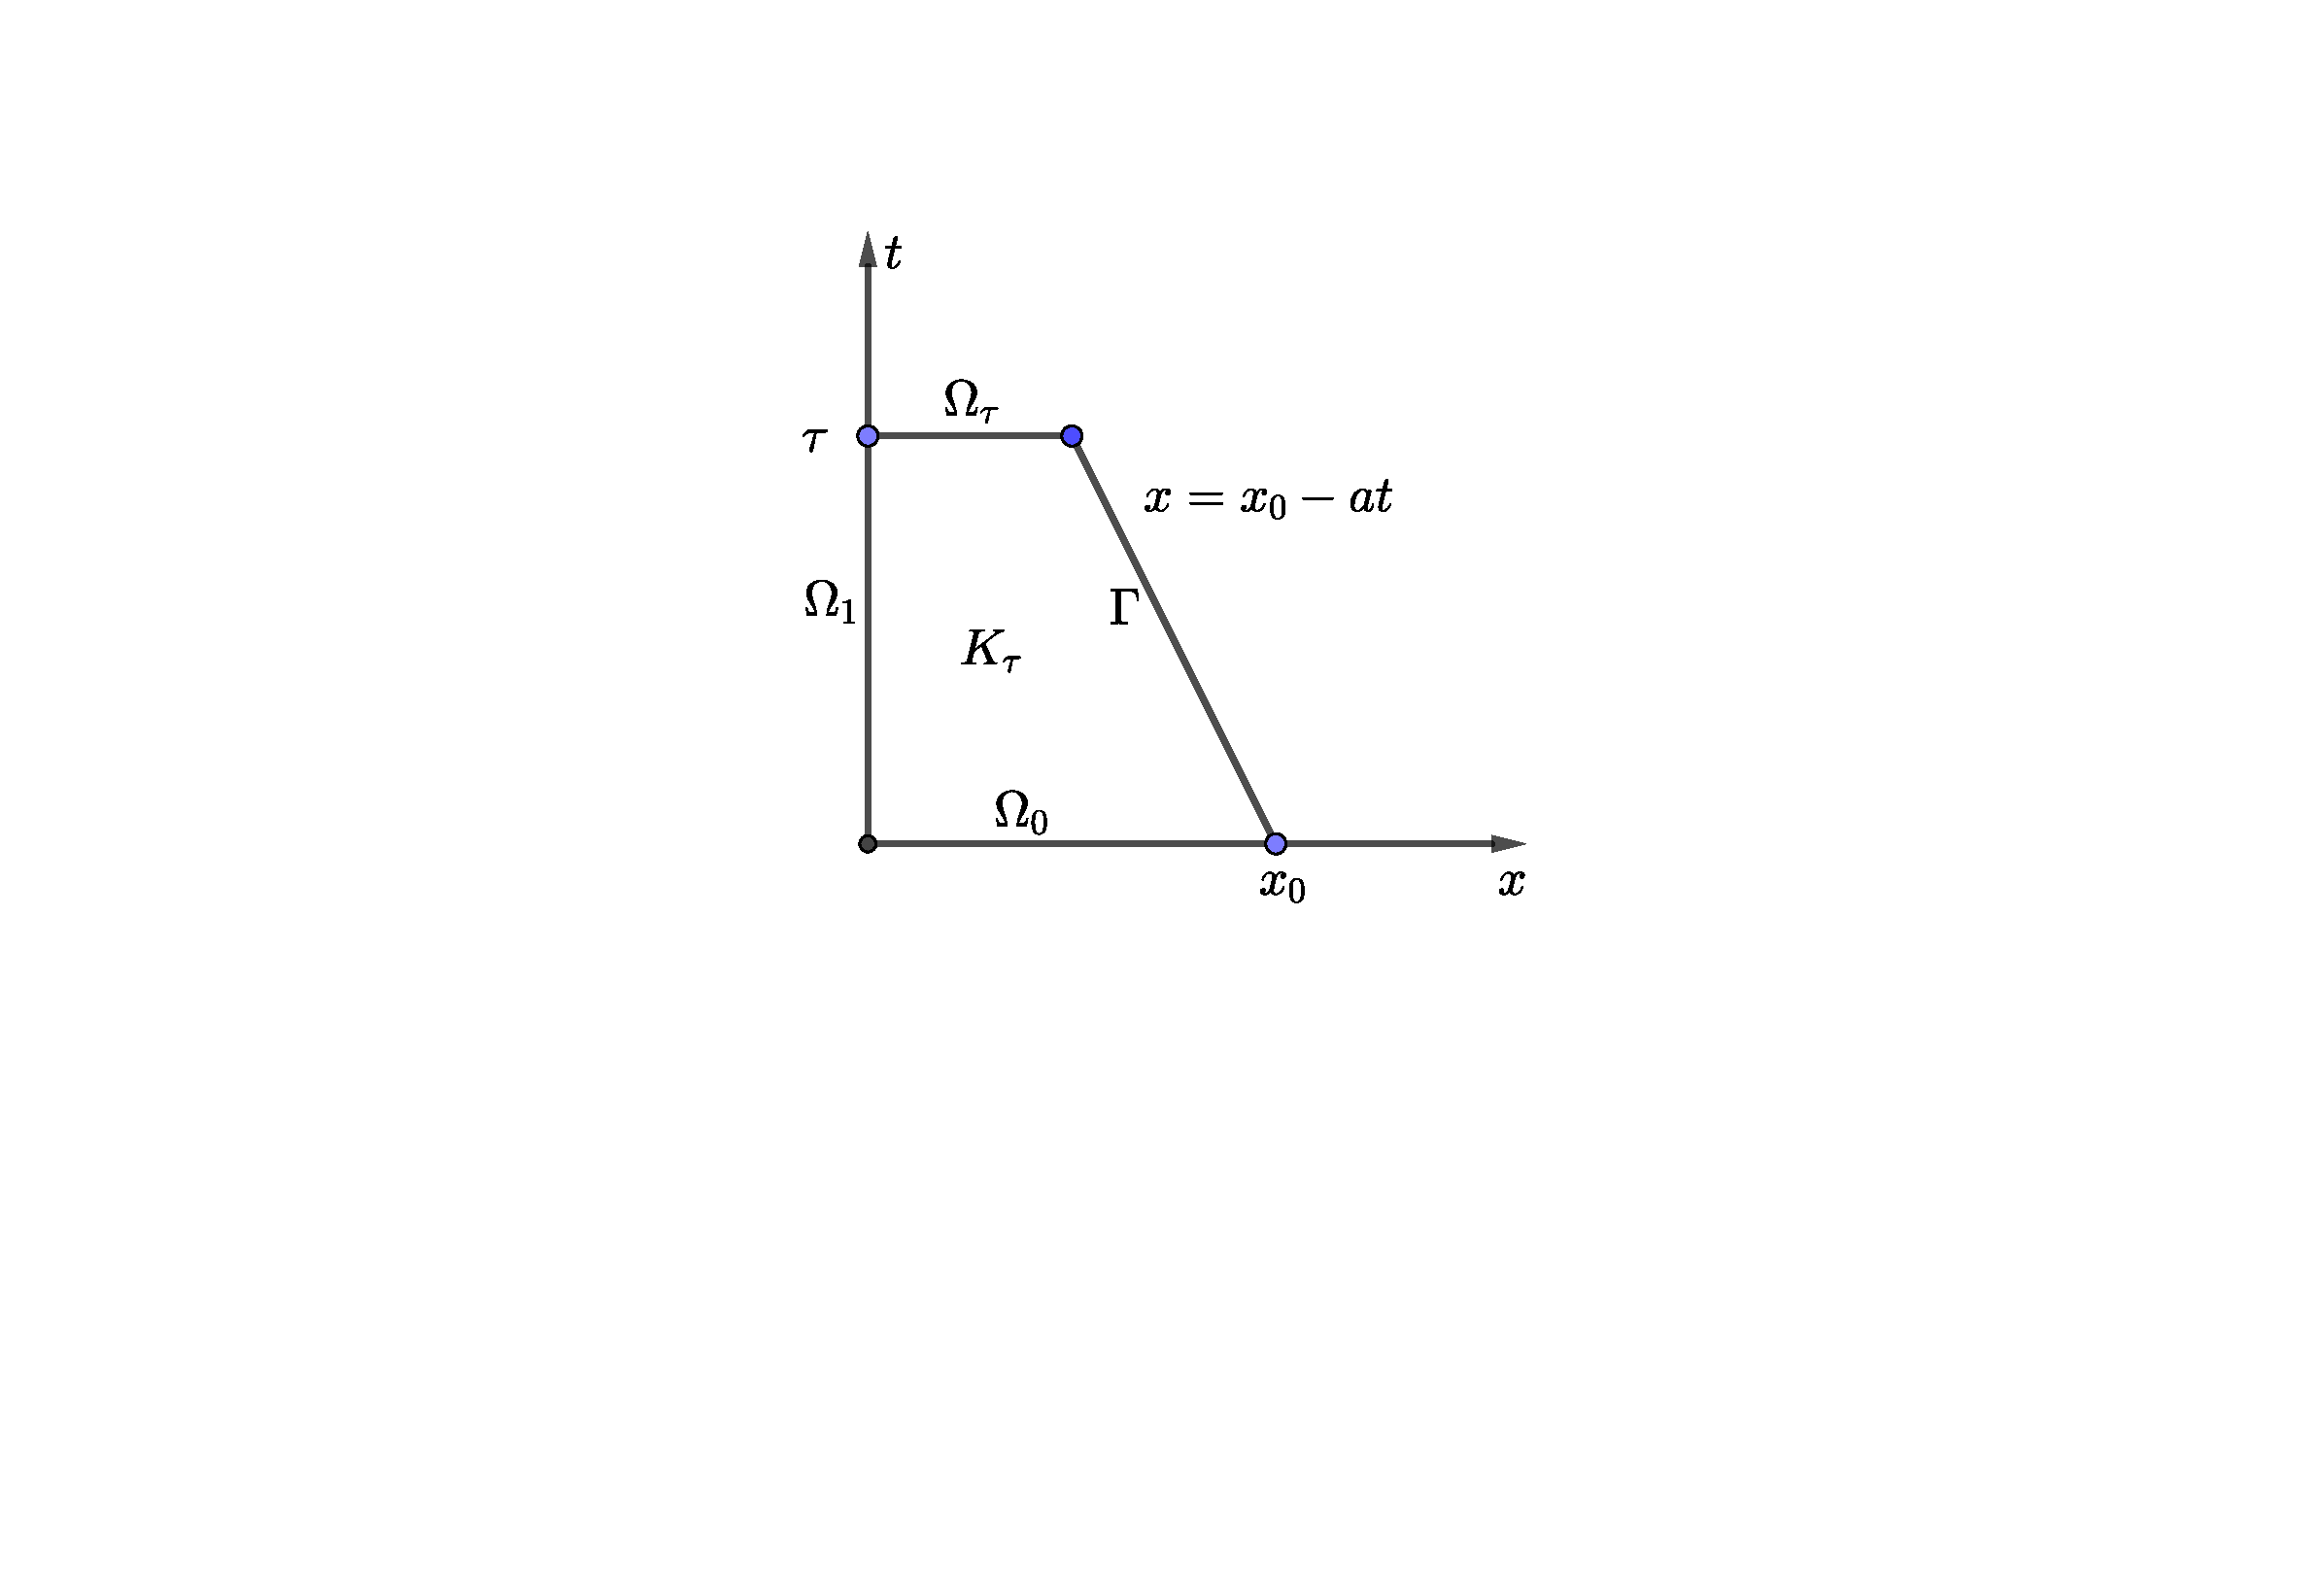
\includegraphics[scale=0.4]{PDEs证明波动方程半平面问题解的唯一性.pdf}
    \end{figure}

    考虑对波动方程进行变换
    \begin{align*}
        \int_{K_\tau}\frac{\partial u}{\partial t}\left(\frac{\partial^2u}{\partial t^2}-a^2\frac{\partial^2 u}{\partial x^2}\right)\,\d x\,\d t = \int_{K_\tau}\frac{\partial u}{\partial t}f(x, t)\,\d x\,\d t.
    \end{align*}
    对左式进行化简
    \begin{align*}
        \text{左式} =&\ \int_{K_\tau}\left\{\frac{1}{2}\frac{\partial}{\partial t}\left((\frac{\partial u}{\partial t})^2+a^2(\frac{\partial u}{\partial x})^2\right)-a^2\frac{\partial}{\partial x}(\frac{\partial u}{\partial x}\,\frac{\partial u}{\partial t})\right\}\,\d x\,\d t\\
        \xlongequal{\text{Green公式}}&\ -\int_{\partial K_\tau}\frac{1}{2}\left((\frac{\partial u}{\partial t})^2+a^2(\frac{\partial u}{\partial x})^2\right)\,\d x+a^2(\frac{\partial u}{\partial x}\,\frac{\partial u}{\partial t})\,\d t\\
        =&\ \int_{\Omega_\tau}\frac{1}{2}(u_t^2+a^2u_x^2)\,\d x-\int_{\Omega_0}\frac{1}{2}(\psi^2+a^2\varphi_x^2)\,\d x+\int_{\Omega_1}a^2\mu_x\mu_t\,\d t-\int_{\Gamma}\frac{1}{2}(u_t^2+a^2u_x^2)\,\d x+a^2(u_xu_t)\,\d t.
    \end{align*}
    在$\Gamma$上有$\d x=-a\,\d t$,则右式第四项等于$\int_0^{\tau}\frac{a}{2}(u_t+au_x)^2\,\d t\geq 0$.
    
    由于$\int_{K_\tau}2u_tf\,\d x\,\d t\leq \int_{K_\tau}u_t^2\,\d x\,\d t+\int_{K_\tau}f^2\,\d x\,\d t$,于是有
    \begin{equation*}
        \int_{\Omega_\tau}(u_t^2+a^2u_x^2)\,\d x\leq \int_{\Omega_0}(\psi^2+a^2\varphi_x^2)\,\d x-2\int_{\Omega_1}a^2\mu_x\mu_t\,\d t+\int_{K_\tau}f^2\,\d x\,\d t+ \int_{K_\tau}u_t^2\,\d x\,\d t
    \end{equation*}

    令$G(\tau) = \int_{K_\tau}(u_t^2+a^2u_x^2)\,\d x = \int_0^\tau\int_{\Omega_\tau}(u_t^2+a^2u_x^2)\,\d x\,\d t$,所以有$G(0) = 0$且
    \begin{equation*}
        \frac{\d G(\tau)}{\d\tau}\leq G(\tau)+F(\tau)
    \end{equation*}
    其中$F(\tau) = \int_{\Omega_0}(\psi^2+a^2\varphi_x^2)\,\d x-2\int_{\Omega_1}a^2\mu_x\mu_t\,\d t+\int_{K_\tau}f^2\,\d x\,\d t$. \add 由Gronwall不等式可知$G(\tau)\leq MF(\tau)$,于是可得到类似能量不等式结果
    \begin{equation*}
        \int_{\Omega_\tau}(u_t^2+a^2u_x^2)\,\d x \leq M_1\left(\int_{\Omega_0}(\psi^2+a^2\varphi_x^2)\,\d x-2\int_{\Omega_1}a^2\mu_x\mu_t\,\d t+\int_{K_\tau}f^2\,\d x\,\d t\right)
    \end{equation*}
    
    进一步,可得到能量模估计
    \begin{equation*}
        \int_{\Omega_\tau}u^2(x,\tau)\,\d x\leq M_2\left(\int_{\Omega_0}(\varphi^2+\psi^2+a^2\varphi_x^2)\,\d x-2\int_{\Omega_1}a^2\mu_x\mu_t\,\d t+\int_{K_\tau}f^2\,\d x\,\d t\right)
    \end{equation*}
    不难得到,当$\varphi=\psi=\mu=f=0$时,该问题只有零集,所以上式说明了该问题解的唯一性.
\end{solution}
\begin{problem}
    证明以下Cauchy问题
    \begin{equation*}
        \begin{cases}
            u_{tt}-a^2u_{xx}+b(x,t)u_x+c(x,t)u_t=f(x,t),&\quad x\in\R,t > 0,\\
            u|_{t=0} = \varphi(x),\ u_t|_{t=0}=\psi(x),&\quad x\in\R
        \end{cases}
    \end{equation*}
    解的唯一性,其中$b(x,t),\ c(x,t)$都是有界连续函数.
\end{problem}
\begin{solution}
    类似于能量不等式证明,首先对第一式左右同乘$u_t$,再在$K_\tau$上进行积分可得
    \begin{equation*}
        \int_{K_\tau}\left\{\frac{1}{2}\frac{\partial}{\partial t}(u_t^2+a^2u_x^2)-a^2\frac{\partial}{\partial x}(u_xu_t)\right\}\,\d x\,\d t+\int_{K_\tau}b(x,t)u_xu_t+c(x,t)u_t^2\,\d x\,\d t=\int_{K_\tau}u_tf\,\d x\,\d t.
    \end{equation*}
    对左式第一项进行变化并使用Green公式转化为第二型曲线积分,再证明$J_3\geq 0$,于是可得
    \begin{equation*}
        \int_{\Omega_\tau}(u_t^2+a^2u_x^2)\,\d x\leq \int_{\Omega_0}(\psi^2+a^2\varphi_x^2)\,\d x-2\int_{K_\tau}(b(x,t)u_xu_t+c(x,t)u_t^2)\,\d x\,\d t+\int_{K_\tau}u_t^2\,\d x\,\d t+\int_{K_\tau}f^2\,\d x\,\d t.
    \end{equation*}
    由于$b(x, t),\ c(x,t)$有界,不妨令$C = \sup_{(x,t)\in K_\tau}2|b(x,t)|+2|c(x,t)|$,$C_0 = \max\{\frac{C}{a^2},2C\}$,于是
    \begin{align*}
        -2\int_{K_\tau}(b(x,t)u_xu_t+c(x,t)u_t^2)\,\d x\,\d t\leq C\int_{K_\tau}(u_xu_t+u_t^2)\,\d x\,\d t\leq&\ \int_{K_\tau}C(2u_t^2+u_x^2)\,\d x\,\d t\\
        \leq&\ \int_{K_\tau}C_0(u_t^2+a^2u_x^2)\,\d x\,\d t.
    \end{align*}

    记$G(\tau) = \int_{K_\tau}(u_t^2+a^2u_x^2)\,\d x\,\d t,\ F(\tau) = \int_{\Omega_0}(\psi^2+a^2\varphi_x^2)\,\d x+\int_{K_\tau}f^2\,\d x\,\d t$,于是有
    \begin{equation*}
        \frac{\d G(\tau)}{\d \tau}\leq (C_0+1)G(\tau)+F(\tau)
    \end{equation*}
    由Gronwall不等式可知$G(\tau)\leq MF(\tau)$,于是可以得到能量不等式,进一步,可以得到能量模不等式,从而说明该Cauchy问题具有唯一解.
\end{solution}
\begin{problem}
    试问下述半无界问题
    \begin{equation*}
        \begin{cases}
            u_{tt}-u_{xx}+u_t+u_x=0,&\quad x > 0, t > 0,\\
            u|_{x=0} = 0,&\quad t\geq 0,\\
            u|_{t=0}=\varphi(x),\ u_t|_{t=0} = \psi(x),&\quad x\geq 0
        \end{cases}
    \end{equation*}
    能否直接用对称开拓法求解?为什么?试用特征线法求解.
\end{problem}
\begin{solution}
    通过下属求解解的表达式可知,该问题的解无法保证与$\varphi,\psi$保持相同的奇偶性,因此无法使用对称开拓法进行求解. 下面使用特征线法进行求解.\add 

    由于$\left(\frac{\partial^2}{\partial t^2}-\frac{\partial^2}{\partial x^2}+\frac{\partial}{\partial t}+\frac{\partial}{\partial x}\right) = \left(\frac{\partial}{\partial t}-\frac{\partial}{\partial x}+1\right)\left(\frac{\partial}{\partial t}+\frac{\partial}{\partial x}\right)$. \add 令$u_t+u_x = v$,则上述半平面问题等价于求解
    \begin{equation*}
        \begin{cases}
            u_t+u_x=v,\\
            u|_{x=0} = 0,\\
            u(x,0) = \varphi(x).
        \end{cases}(1)\qquad\begin{cases}
            v_t-v_x = -v,\\
            v(x,0) = u_t(x,0)+u_x(x,0) = \psi(x)+\varphi'(x).
        \end{cases}(2)
    \end{equation*}
    先求解$(2)$式,令$\begin{cases}
        \frac{\d x(t)}{\d t} = -1,\\
        x(0) = c.
    \end{cases}$ 则$x = -t+c,\ c = x+t$,方程$(2)$转化为$\frac{\d v}{\d t} = -v$,于是
    \begin{equation*}
        v = (\psi(c)+\varphi'(c))\e^{-t} = (\psi(x+t)+\varphi'(x+t))\e^{-t},
    \end{equation*}
    再求解方程$(1)$,令$\begin{cases}
        \frac{\d x(t)}{\d t} = 1,\\ x(0) = c.
    \end{cases}$则$x = t+c,\ c= x-t$,方程$(1)$转化为$\frac{\d u}{\d t} = (\psi(x+t)+\varphi'(x+t))\e^{-t}$,由于$x>0,t>0$,分两类情况讨论,当$x\geq t$时
    \begin{align*}
        u =&\ \varphi(x(0)) +\int_0^t\{\psi(x(\tau)+\tau)+\varphi'(x(\tau)+\tau)\}\e^{-\tau}\,\d \tau\\
        =&\ \varphi(c)+\int_0^t\{\psi(c+2\tau)+\varphi'(c+2\tau)\}\e^{-\tau}\,\d \tau\\
        \xlongequal{\xi = c+2\tau}&\ \varphi(c)+\frac{1}{2}\int_{c}^{c+2t}\{\psi(\xi)+\varphi'(\xi)\}\e^{-\frac{\xi-c}{2}}\,\d \xi\\
        =&\ \varphi(x-t)+\frac{1}{2}\int_{x-t}^{x+t}\{\psi(\xi)+\varphi'(\xi)\}\e^{-\frac{\xi-x+t}{2}}\,\d \xi\\
        =&\ \frac{1}{2}\varphi(x-t)+\frac{1}{2}\varphi(x+t)\e^{-t}+\frac{1}{2}\int_{x-t}^{x+t}\{\psi(\xi)+\varphi(\xi)\}\e^{-\frac{\xi-x+t}{2}}\,\d \xi
    \end{align*}
    当$0\leq x < t$时
    \begin{align*}
        u =&\ \int_{t-x}^t\{\psi(x(\tau)+\tau)+\varphi'(x(\tau)+\tau)\}\e^{-\tau}\,\d \tau\\
        =&\ \int_{t-x}^t\{\psi(c+2\tau)+\varphi'(c+2\tau)\}\e^{-\tau}\,\d \tau\\
        \xlongequal{\xi = c+2\tau}&\ \frac{1}{2}\int_{c+2t-2x}^{c+2t}\{\psi(\xi)+\varphi'(\xi)\}\e^{-\frac{\xi-c}{2}}\,\d \xi\\
        =&\ \frac{1}{2}\int_{t-x}^{t+x}\{\psi(\xi)+\varphi'(\xi)\}\e^{-\frac{\xi-x+t}{2}}\,\d \xi\\
        =&\ \frac{1}{2}\varphi(x+t)\e^{-t}-\frac{1}{2}\varphi(t-x)\e^{-t+x}+\frac{1}{2}\int_{t-x}^{x+t}\{\psi(\xi)+\varphi(\xi)\}\e^{-\frac{\xi-x+t}{2}}\,\d \xi
    \end{align*}
\end{solution}
\begin{problem}
    求解古尔沙问题
    \begin{equation*}
        \begin{cases}
            u_{tt} = u_{xx},&\quad t > |x|,\\
            u|_{t=-x}=\varphi(x),&\quad x \leq 0,\\
            u|_{t=x} = \psi(x),&\quad x\geq 0,
        \end{cases}
    \end{equation*}
    其中$\varphi(0) = \psi(0)$. 如果$\varphi(x)$给定在$(-a,0]$,$\psi(x)$给定在$[0,b]$,指出此定解条件的决定区域.
\end{problem}
\begin{solution}
    使用行波法求解,令$\begin{cases}
        \xi = x-t,\\
        \eta = x+t.
    \end{cases}$则$_{tt}=u_{xx}\Rightarrow u_{\xi\eta} = 0\Rightarrow u = F(\xi)+G(\eta) = F(x-t)+G(x+t)$.

    当$x\leq 0$时,$u|_{t=-x} = u(x,-x) = F(2x)+G(0) = \varphi(x)$.

    当$x\geq 0$时,$u|_{t=x} = F(0)+G(2x)=\psi(x)$. 且$F(0)+G(0) = \varphi(0) = \psi(0)$.\add

    于是$\begin{cases}
        F(x) = \varphi(\frac{x}{2})-G(0),\\
        G(x) = \psi(\frac{x}{2})-F(0).
    \end{cases}\Rightarrow u = \varphi(\frac{x-t}{2})+\psi(\frac{x+t}{2})-\varphi(0)$.\add

    当给定$\varphi$在$(-a,0]$,$\psi$在$[0,b]$,于是决定区域为
    \begin{equation*}
        \begin{cases}
            -a < \frac{x-t}{2}\leq 0,\add\\
            0\leq \frac{x+t}{2}\leq b.
        \end{cases}\Rightarrow \begin{cases}
            x\leq t < x+2a,\\
            -x\leq t\leq 2b-x.
        \end{cases}
    \end{equation*}
\end{solution}
% 下面给一些功能的写法
\iffalse
% 图片模板
\centerline{
    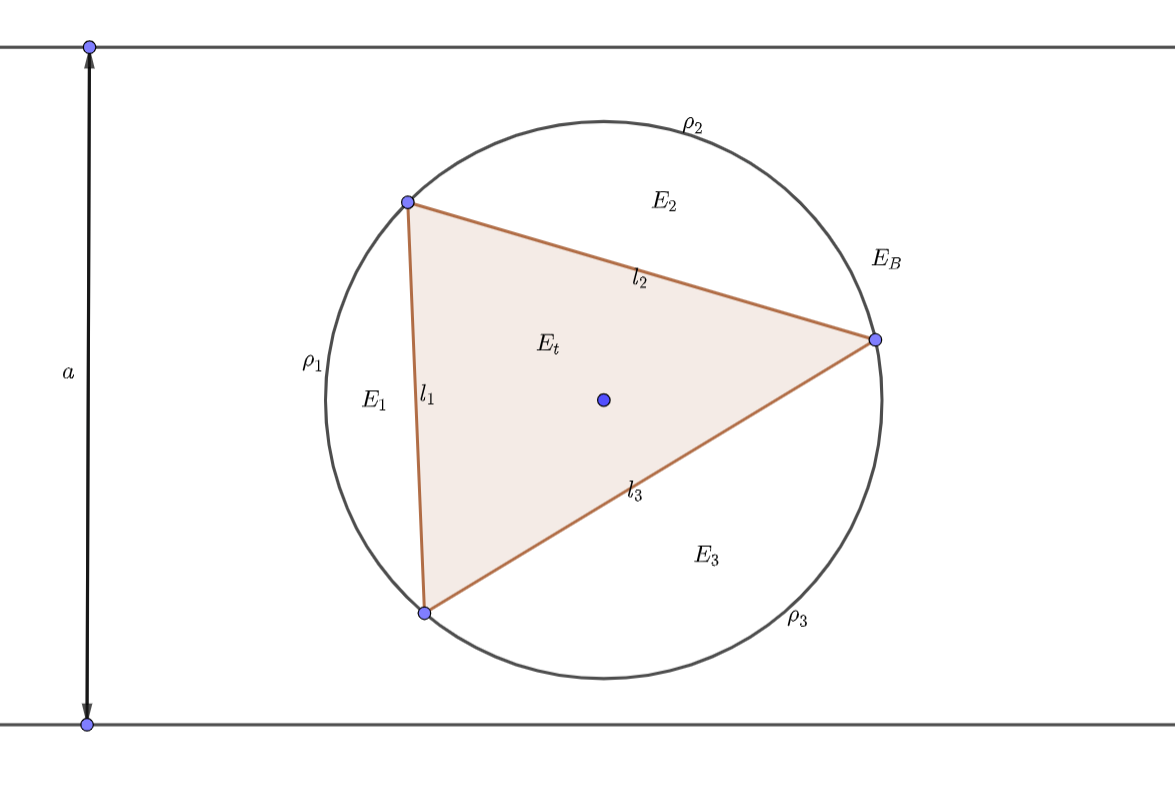
\includegraphics[width=0.8\textwidth]{figure.png}
}
% 表格模板
\renewcommand\arraystretch{0.8} % 设置表格高度为原来的0.8倍
\begin{table}[!htbp] % table标准
    \centering % 表格居中
    \begin{tabular}{p{1cm}<{\centering}p{1cm}<{\centering}p{3cm}<{\centering}p{5cm}<{\centering}} % 设置表格宽度
    %\begin{tabular}{cccc}
        \toprule
        $x_i$ & $f[x_1]$ & $f[x_i,x_{i+1}]$ & $f[x_i,x_{i+1},x_{i+2}]$ \\
        \midrule
        $x_0$ & $f(x_0)$ &                  &                          \\
        $x_0$ & $f(x_0)$ & $f'(x_0)$        &                          \\
        $x_0$ & $f(x_1)$ & $\frac{f(x_1)-f(x_0)}{x_1-x_0}$ & $\frac{f(x_1)-f(x_0)}{(x_1-x_0)^2}-\frac{f'(x_0)}{x_1-x_0}$\\
        \bottomrule
    \end{tabular}
\end{table}

\def\Log{\text{Log}} % 一个简单的宏定义
$\Log$ % 调用方法
\fi

\end{document}